\documentclass{article}
\usepackage{algpseudocode,extramarks,fancyhdr,paralist,amsmath,amsthm,amssymb,mathtools,url,graphicx,pdfpages,tikz,pdfpages,rotating,mathtools, hyperref, bm, hyperref,amsfonts,pgf,mathrsfs,xcolor,comment,mathdots,braket,physics,graphicx}
\usepackage[plain]{algorithm}
\usepackage[utf8]{inputenc}
\usepackage[left=1in,right=1in,top=1.2in, bottom=1in]{geometry}

\usetikzlibrary{automata,positioning,decorations.pathreplacing,decorations.markings,calc}

%
% Basic Document Settings
%

\topmargin=-0.45in
\evensidemargin=0in
\oddsidemargin=0in
\textwidth=6.5in
\textheight=9.0in
\headsep=0.25in

\linespread{1.1}

\pagestyle{fancy}
\lhead{\hmwkAuthorName}
\chead{\hmwkClass\ : \hmwkTitle}
\rhead{\firstxmark}
\lfoot{\lastxmark}
\cfoot{\thepage}

\newcommand{\dx}{\mathrm{d}x}
\newcommand{\dy}{\mathrm{d}y}
\newcommand{\dt}{\mathrm{d}t}
\newcommand{\solution}{\textbf{\large Solution}}
\newcommand{\E}{\mathrm{E}}
\newcommand{\Var}{\mathrm{Var}}
\newcommand{\Cov}{\mathrm{Cov}}
\newcommand{\Bias}{\mathrm{Bias}}
\newcommand{\lp}{\left(}
\newcommand{\rp}{\right)}
\newcommand{\bvec}{\vectorbold}
\newcommand{\di}{\mathrm{d}}
\setlength\parindent{0pt}
\newcommand{\uv}[1]{\hat{\bvec{#1}}}
\renewcommand{\grad}{\bvec{\nabla}}
\newcommand{\lap}{\bvec{\nabla}^2}
\renewcommand{\part}[2]{\partial_{#1}\left[ #2 \right]}
\newcommand{\bpart}[2]{\left[ #1 \right]_{#2}}
\newcommand{\bg}[1]{\begin{gather*} #1
\end{gather*}}
\newcommand{\lag}{\mathcal{L}}
\newcommand{\ham}{\mathcal{H}}


%
%Proof and theorem structure
%

\theoremstyle{definition} 
\newtheorem{theorem}{Theorem}
\newtheorem{lemma}[theorem]{Lemma}
\newtheorem{claim}[theorem]{Claim}
\newtheorem{corollary}[theorem]{Corollary}
\newtheorem{conjecture}[theorem]{Conjecture}
\newtheorem{definition}[theorem]{Definition}
\newtheorem{example}[theorem]{Example}
\newtheorem{remark}[theorem]{Remark}
\newtheorem{important}[theorem]{Important Note}
\newtheorem{recall}[theorem]{Recall}
\newtheorem{note}[theorem]{Note}
\newtheorem{question}[theorem]{Question}
\newtheorem*{definition*}{Definition}
\newtheorem*{theorem*}{Theorem}
\newtheorem*{claim*}{Claim}

%
%Prefreable integration method
%

\def\upint{\mathchoice%
    {\mkern13mu\overline{\vphantom{\intop}\mkern7mu}\mkern-20mu}%
    {\mkern7mu\overline{\vphantom{\intop}\mkern7mu}\mkern-14mu}%
    {\mkern7mu\overline{\vphantom{\intop}\mkern7mu}\mkern-14mu}%
    {\mkern7mu\overline{\vphantom{\intop}\mkern7mu}\mkern-14mu}%
  \int}
\def\lowint{\mkern3mu\underline{\vphantom{\intop}\mkern7mu}\mkern-10mu\int}

%
% Create Problem Sections
%

\newcommand{\enterProblemHeader}[1]{
    \nobreak\extramarks{}{Problem \arabic{#1} continued on next page\ldots}\nobreak{}
    \nobreak\extramarks{Problem \arabic{#1} (continued)}{Problem \arabic{#1} continued on next page\ldots}\nobreak{}
}

\newcommand{\exitProblemHeader}[1]{
    \nobreak\extramarks{Problem \arabic{#1} (continued)}{Problem \arabic{#1} continued on next page\ldots}\nobreak{}
    \stepcounter{#1}
    \nobreak\extramarks{Problem \arabic{#1}}{}\nobreak{}
}

\setcounter{secnumdepth}{0}
\newcounter{partCounter}
\newcounter{homeworkProblemCounter}
\setcounter{homeworkProblemCounter}{1}
\nobreak\extramarks{Problem \arabic{homeworkProblemCounter}}{}\nobreak{}

%
% Homework Problem Environment
%
% This environment takes an optional argument. When given, it will adjust the
% problem counter. This is useful for when the problems given for your
% assignment aren't sequential. See the last 3 problems of this template for an
% example.
%
\newenvironment{homeworkProblem}[1][-1]{
    \ifnum#1>0
        \setcounter{homeworkProblemCounter}{#1}
    \fi
    \section{Problem \arabic{homeworkProblemCounter}}
    \setcounter{partCounter}{1}
    \enterProblemHeader{homeworkProblemCounter}
}{
    \exitProblemHeader{homeworkProblemCounter}
}

%
% Homework Details
%   - Title
%   - Due date
%   - Class
%   - Section/Time
%   - Instructor
%   - Author
%
%----------------------------------------------------------------------------------------------------------------------------------------------------------------------------------
%----------------------------------------------------------------------------------------------------------------------------------------------------------------------------------
\newcommand{\hmwkTitle}{Homework\ \#3}
\newcommand{\hmwkDueDate}{Fri. Oct. 8th}
\newcommand{\hmwkClass}{Classical Mechanics}
\newcommand{\hmwkAuthorName}{\textbf{Harlan Heilman}}
%----------------------------------------------------------------------------------------------------------------------------------------------------------------------------------
%----------------------------------------------------------------------------------------------------------------------------------------------------------------------------------
%
% Title Page
%

\title{
    \vspace{2in}
    \textmd{\textbf{\hmwkClass\ }}\\
    \textmd{\textbf{\hmwkTitle\ }}\\
    \normalsize\vspace{0.1in}\small{Due\ on\ \hmwkDueDate\ }\\
    \vspace{3in}
}

\author{\hmwkAuthorName}
\date{}

%----------------------------------------------------------------------------------------------------------------------------------------------------------------------------------
%----------------------------------------------------------------------------------------------------------------------------------------------------------------------------------
%----------------------------------------------------------------------------------------------------------------------------------------------------------------------------------

\begin{document}

\maketitle

\pagebreak

\begin{homeworkProblem}
    Consider a bead of mass $m$ sliding down a wire from the point $\vec{P} = (x_0, y_0)$.
    \begin{itemize}

    \item[1] Write and expression for the total time $T$ it takes for the bead to slide from $\vec{P}$ to the origin as a functional of the path of the wire $y(x)$.


    \item[2] Write the Euler-Lagrange equations for the solution.


    \item[3] Show that the solution is a cycloid (or solve the problem directly).
    \end{itemize}
    \textbf{Solution}
    Let us start off with a picture showing the two points and some possible paths between the points
    \begin{figure}[h]
        \centering
        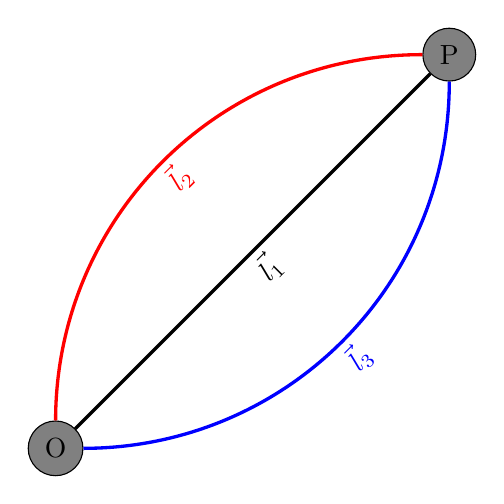
\begin{tikzpicture}
        \tikzset{vertex/.style={draw,shape=circle,fill=gray}, el/.style = {inner sep=2pt, align=left, sloped},every label/.append style = {font=\tiny}}
            \node[vertex] (O) at (0,0) {O};
            \node[vertex] (P) at (5,5) {P};
            \draw (P) edge [very thick, black] [el, below]node{$\vec{l_1}$} (O);
            \draw (P) edge [bend right=45, very thick, red] [el,below]node{$\vec l_2$} (O);
            \draw (P) edge [bend left= 45,very thick, blue] [el, below]node{$\vec l_3$} (O);
        \end{tikzpicture}
    \end{figure}
    \\
    Here $l_1,l_2$, and $l_3$ rep-present different possible paths that the bead could take to get from $P$ to $O$. \\
    
    \textbf{Part (a)}\\
    We begin by stating that the distance any bead will travel is nothing but 
    \[
        l = \int_{P}^{O}\mathrm{d}l = \int_P^O\sqrt{1+y'^2}\dy
    \]
    Thus we know that the time it takes for the bead to get from $P$ to $O$ is nothing but 
    \[
        T = l/v = \int_P^Ov^{-1}\sqrt{1+y'^2}\dy
    \]
    But we know that the velocity of the bead will be dependent on its initial velocity, and the shape of the path that it takes. But if we restrict the problem to bead at rest at time $t = 0$, we have the initial energy of the system as $E_i = mgy_0$. But after some time later, the beads energy is nothing but $E_t = \frac{1}{2}mv^2+mgy$. Thus we have an equation for the beads velocity as 
    \[
        v = \sqrt{2g(y_0-y)}
    \]
    This makes sense as in its initial position, $y = y_0$, and we have no velocity for the bead. Thus we have an equation for the time it takes for the particle to travel down the wire as 
    \[
        T = \int_P^O(\sqrt{2g(y_0-y)})^{-1}\sqrt{1+y'^2}\dy
    \]
    \textbf{Part (b)}\\
    But now we want to minimise the time it takes and come to some variational principle 
    \[
        \delta T[y,x] = 0
    \]
    But we can cheat a bit and turn straight to the Euler-Lagrange equations, as we know that this is time integral is analogous to an action integral. This means that we can say 
    \[
        \mathcal{L}'[y,y',x] = (\sqrt{2g(y_0-y)})^{-1}\sqrt{1+y'^2}
    \]
    Thus we have the various "momentum" as
    \begin{align*}
         \frac{\partial\lag}{\partial x} =0 &\implies P'_x = \part{x}{\lag} = constant\\
         \frac{\partial\lag}{\partial y} = 1 &;\ P'_y = \part{y}{\lag} =  y'(1+y'^2)^{-1/2}(2g(y_0-y))^{-1/2}
    \end{align*}
    But since $x$ does not appear in our "Lagrangian", we know that the equivalent of a Hamiltonian is conserved. This means that we have
    \[
        \part{x}{-\ham}= \part{x}{\lag' - y'\part{y'}{\lag}} = 0 \implies \lag' - y'\part{y'}{\lag}
    \]
    Calculating the partial derivative of $\lag'$ gives us
    \[
        \part{y'}{\lag} = y'(1+y'^2)^{-1/2}(2g(y_0-y))^{-1/2}
    \]
    Since the "Hamiltonian" is constant, we shall set it equal to some scalar $c$, and thus we have the equation
    \[
        c = \frac{\sqrt{1+(y')^2}}{\sqrt{2g(y_0-y)}} - \frac{y'^2}{\sqrt{(1+y'^2)(2g(y_0-y))}}
    \]
    Let $a = 1/2gc^2$, we now do a little bit of simplification in squaring both sides and we are left with the separable differential equation
    \[
        \dx = \frac{\sqrt{(y_0-y)}}{\sqrt{a - y_0-y}}\dy
    \]
    we introduce the trig substitution of $y = y_0 - a\sin^2(\theta/2)$, where $\dy = -a\sin(\theta/2)\cos(\theta/2)\mathrm{d}\theta$ (this guess was made by knowing what the parametric equations for a cycloid look like and verifying that they allow us to solve the integral, in this case they do). We note that $\sin^2(\theta/2) = 1/2(1-\cos(\theta )$ and this allows us to integrate getting the parametric equation for $x$ as
    \[
        x = \frac{a}{2}(\theta - \sin(\theta))+k
    \]
    where $k$ is some constant of integration, and $a$ is defined above. We use our substitution for $y$ that was needed for integration, and get the $y$ parametric equation as
    \[
        y = y_0 +\frac{a}{2}(1-\cos(\theta))
    \]
    We will check that our substitution satisfies the conditions for stationary points at the end. But now we input the boundary conditions, $x = x_0 \iff y = y_0$, and $x = 0 \iff y = 0$. When $y = y_0$, we have $\theta = 0$, and thus $k = x_0$. For the last one, $x=0$, and $y=0$, we have the set of nonlinear equations 
    \begin{align*}
        -2x_0 &= a(\theta_0 - \sin(\theta_0)\\
        -2y_0 &=a(1-\cos(\theta_0)
    \end{align*}
    where $a$ and $\theta_0$ are unknown. Now we will solve this numerically in part c, but here let us look at the units to guess what constants are included in $a$. We know from above, that the units on $a$ must be in terms of length. So we out of the constants in the problem, there are only two that involve only length. These being $x_0$, and $y_0$. Thus there are three possible combinations to get to the constant $a$, i.e. 
    \begin{align*}
        a & \propto \sqrt{x_0y_0}& a & \propto x_0 & a & \propto y_0
    \end{align*}
    However, most likely the one including both parameters will be the case. 
    
    Nonetheless, the parametric equations are 
    \begin{align*}
        x &= x_0 +\frac{a}{2}(\theta - \sin(\theta))\\
        y &= y_0 +\frac{a}{2}(1-\cos(\theta))
    \end{align*}
    \\
    
    \textbf{Part (c)}\\
    Firstly, these are the parametric equations for a cycloid, but to explicitly show this, we need to find out what $a$ is. Do do this, lets set out initial conditions to $x_0 = y_0 = .5$m in line with some of the demo brachistochrone ramps found online. In doing so, I made the following Jupiter notebook to solve for $a$, and the 
    \begin{verbatim}
        from numpy import *
        from scipy.optimize import fsolve
        import matplotlib.pyplot as plt
        import numpy as np
        x0 = .5
        y0 = .5
        def myFunction (z):
            a = z[0]
            t = z[1]
    
            F = empty((2))
            F[0] = x0 + a*(t - np.sin(t))
            F[1] = y0 + a*(1 - np.cos(t))
            return F
        zGuess = array([1,1])
        z = fsolve(myFunction,zGuess)
        print(z)
        [-0.28645852  2.41201114]
        A = z[0]
        theta = np.linspace(0,z[1],100)
        x = x0 + A*(theta - np.sin(theta))
        y = y0 + A*(1 - np.cos(theta))
        f = plt.figure()
        plt.plot(x,y)
        plt.title('Brachistochrone for $x_0 = y_0 = .5$m', fontsize=11)
        plt.xlabel('$y$(m)')
        plt.ylabel('$x$(m)')
        plt.show()
    \end{verbatim}
    So, we see that $a = -0.28645852$, which isn't exactly what we predicted it to be based on dimensional analysis. Now these equations are exactly the equations of a cycloid,
    \begin{align*}
        x = r(t-\sin(t))\\
        y = r(1-cos(t))
    \end{align*}
    except in our equation, the coordinates have undergone the transformation $x \to x-x_0$, and $y\to y-y_0$. However, we also have an issue with the sign on our $a$ most likely. I'm not sure where that came from, but thinking about the problem, this could have come form the bounds. Instead of the bead starting at the origin and rolling in the positive x direction, we see it start at $P$ and roll backwards towards the origin. Or if we imagined $P$ was the origin, the bead starts at the origin $(0,0)$ and rolls backwards towards $(-x_0,-y_0)$. Doing this transformation, and instead taking $x\to x+x_0$, and $y\to y+y_0$, we see that we get $a = 0.28645852$. None the less, here is a graph showing the Brachistochrone.
    \begin{figure}[h]
        \centering
        \includegraphics{brachistochrone.pdf}
        \label{fig:my_label}
    \end{figure}
    \\
    Looking now at this graph, we see that it looks like an upside down cycloid, leading credence to the negative value of $a$. 
    
\end{homeworkProblem}

\pagebreak

\begin{homeworkProblem}
    Find the maximum of the function $f(x,y) = -x^2-y^2$ subject to the constraint that $(x-x_0)^2 + y^2 = R^2$ using the method of Lagrange multipliers.
    \\
    
    \textbf{Solution}
    Let us define the constraint as 
    \[
        G(x,y) = (x-x_0)^2 - y^2 -R^2 = 0
    \]
    And our function is nothing but 
    \[
        f(x,y) = -x^2-y^2
    \]
    Thus we find the maximum and minimum by solving the following equation
    \[
        \grad(f(x,y) - \lambda G(x,y)) = 0
    \]
    Taking the gradient we get the following as a system of equations
    \begin{eqnarray*}
        2(\lambda x-\lambda x_0 - x) = 0\\
        2y(\lambda-1)=0\\
        (x-x_0)^2 + y^2 = R^2
    \end{eqnarray*}
    Looking at the second equation, we see that we see that $y = 0$, and thus we are left with two points in the domain of the constraint that satisfy the equation
    \[
        y=0 \implies (x-x_0)^2 = R^2 \implies x = R \pm x_0
    \]
    Plugging this into the function, we see that when we take $x = R - x_0$, we get the maximum.
    \\
    
    Intuitively this process is like taking a section of the domain and finding the maximum of the function over that range. But the way I think about these forces in terms of Lagrangian mechanics is a bit different, and involves a statics case. Imagine we had a sloped surface that followed some paraboloid $x^2+y^2$. If we dropped a ball into this curved surface, then we would see the ball fall towards the center. But what if wanted to model a static system where we tethered the ball to some point on the surface with a string. Then we would have the constraint on the system where the ball would fall towards the lowest point while being constrained by the string. These are just the methods I use to visualise these problems.
\end{homeworkProblem}

\pagebreak

\begin{homeworkProblem}
    Derive the equations of motion for a bead of mass $m$ moving on a frictionless circular wire of radius $a$ (problem 3.1 but for now consider the wire to be stationary).  Do this three ways:
    \begin{itemize}
    \item[1.] Use Newtonian mechanics by projecting the forces as appropriate.
    \item[2.] Using the Euler-Lagrange equations for the coordinate $\theta(t)$ shown in class or in Fig. 16.1 in the book.
    \item[3.] Using the Euler-Lagrange equations for the coordinates $r(t)$ and $\theta(t)$ but introducing the constraint $r(t) = a$ with the method of Lagrange multipliers.  Show how to use this formulation to find an expression for force of constraint exerted by the wire to keep the bead in place.  (I.e. the force you would feel if you were to hold the wire in place while the bead is moving.)
    \item[4.] Derive the equations of motion for the bead if the wire moves up and down with a time-dependent function $h(t)$.  (This is a driven pendulum.  We will analyze it later.)
    \end{itemize}
    
    \textbf{Solution}\\
    
    Let us start off with drawing the circular loop of wire with the bead attached to it. We define $P$ as the location of the bead on the wire, and place the origin at the center of the circle. We will also be using spherical coordinates here and define the angle from the bottom of the sphere
    \\
    
    \begin{figure}[h]
        \centering
        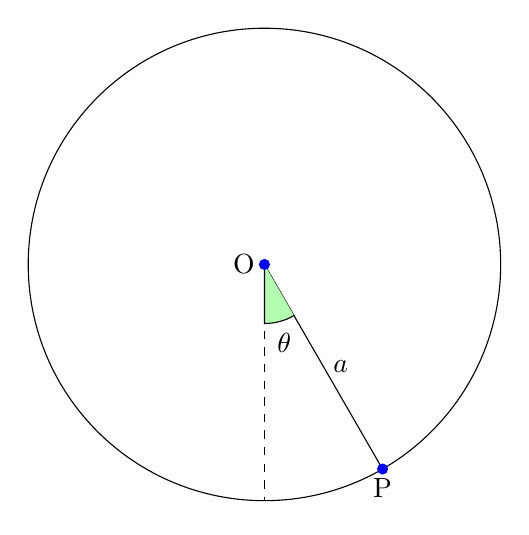
\begin{tikzpicture}
        \coordinate[label=left:{O}] (A) at (0,0);
        \coordinate (B) at (0,-3);
        \coordinate[label=below:{P}] (C) at (3/2,-5.19615242271/2);
        \coordinate[label=right:$a$] (D) at ($ (A)!.5!(C) $);
        
        \draw (A) circle [radius=3];
        \draw[dashed] (A) -- (B);
        \draw (A) -- (C);
        \draw[fill=green!30] (0,0) -- (270:0.75cm) arc (270:300:0.75cm);
        \draw (1/4,-1) node {$\theta$};
        
        \fill[blue] (A) circle [radius = 2pt];
        \fill[blue] (C) circle [radius = 2pt];
        \end{tikzpicture}
    \end{figure}
    \textbf{Part (1)}\\
    Let us start off our analysis using Newton's laws for spherical coordinates. Projected into the plane, these become polar coordinates and we have Newton's second law as
    \begin{align*}
        F_r\uv{r}+F_\theta\uv{\theta} = m(\ddot{r}-r\ddot{\theta})\uv{r}+m(r\dot{\theta}-2\ddot{r}\dot{\theta})\uv{\theta}
    \end{align*}
    But now we must find the net force acting on this bead. To do so, we look at the force diagram
    \begin{figure}[h]
        \centering
        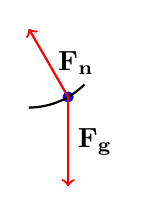
\begin{tikzpicture}
        \coordinate (A) at (0,-1);
        \coordinate (B) at (1/2,-1.73205080757/2);
        
        \coordinate (W) at (1/2,-2);
        \coordinate[label=right:$\bvec{F_g}$] (w) at ($ (B)!.5!(W) $);
        
        \coordinate (N) at (0,0);
        \coordinate[label=right:$\bvec{F_n}$] (n) at ($ (B)!.5!(N) $);
        
        \fill[blue] (B) circle [radius = 2pt];
        \draw[thick] (A) arc (270:315:1);
        \draw[thick, red, ->] (B) -- (W);
        \draw[thick, red, ->] (B) -- (N);
        \end{tikzpicture}
    \end{figure}
    But we know that the normal force points perpendicular to the surface of the wire, so it will all ways be pointing in the opposite direction as $\uv{r}$, i.e., 
    \[
        \bvec{F_n} = -F_n\uv{r}
    \]
    Now we move to projecting the force due to the integration between the bead and the gravitational field of the earth. Assuming that we are near the surface of the earth, we know that $\bvec{F_g} = mg(-\uv{z})$. Thus we project $\bvec{F_g}$ onto the basis vectors $\uv{r}$, and $\uv{\theta}$. In doing so, we find 
    \begin{align*}
        \bvec{F_g}\cdot \uv{r} &= mg\cos\theta\\
        \bvec{F_g}\cdot \uv{\theta} &= -mg\sin\theta
    \end{align*}
    This makes sense as when the bead is at $\theta = \pi/2$, the force of gravity will be pointing in the oposite direction as $\uv{\theta}$, and will have no component in the $\uv{r}$ direction. Plugging this into Newton's 2nd law as defined above, we have
    \begin{align*}
        mg\cos\theta-F_n &= m(\ddot{r}-r\ddot{\theta})\\
        -mg\sin\theta &= m(r\ddot{\theta}-2\dot{r}\dot{\theta})
    \end{align*}
    But we know that the bead is constrained to move only on the wire of fixed radius $r = a$. Thus the first equation is not relevant. Plugging in $a = r$ in the second problem, we get 
    \[
        -g\sin\theta = a\ddot{\theta} \iff \ddot{\theta} = -\frac{g}{a}\sin\theta
    \]
    the equations of motion for a pendulum. 
    \\
    
    \textbf{Part (2)}\\
    Since we know that we want to get back to Newton's laws of motion, we can use the Lagrangian as $\lag = T - V$. But the kinetic energy is nothing but 
    \[
        T = \frac{m}{2}(\dot{r}^2 +r^2\dot{\theta}^2) 
    \]
    But here we have $r = a$ and $\dot{r} = 0$ so the kinetic energy reduces to 
    \[
        T = \frac{m}{2}(a^2\dot{\theta}^2)
    \]
    similarly, the potential is 
    \[
        V = mga(1-\cos\theta) = -mga\cos\theta
    \]
    Where we throw out the $mga$ since we can just set the zero energy as $\theta = \pi/2$ or at a height $a$. This means that that the Lagrangian is nothing but 
    \[
        \lag[\theta,\dot{\theta},t] = \frac{m}{2}(a^2\dot{\theta}^2) + mga\cos\theta
    \]
    While $t$ is cyclic, and the Hamiltonian is conserved, this problem is easier using the Euler-Lagrange equations. So we find
    \[
        P_\theta = \part{\dot{\theta}}{\lag} = ma^2\dot{\theta}
    \]
    But we know that 
    \[
        \dot{P_\theta} = ma^2\ddot{\theta} = \part{\theta}{\lag} = -mga\sin{\theta}
    \]
    and thus we have a familiar equation
    \[
        \ddot{\theta} = -\frac{g}{a}\sin{\theta}
    \]
    the equation of a pendulum.
    \\
    
    \textbf{Part (3)}\\
    What if we where to take the Lagrangian above and introduce a Holonomic constraint $r = a$. We would have the Lagrangian as 
    \[
        \lag[r,\dot{r},\theta,\dot{\theta},t] = \frac{m}{2}(\dot{r}^2+r^2\dot{\theta}^2) +mgr\cos\theta - F_r(r-a)
    \]
    If $r = a$, this reduces to the Lagrangian above. Now we look at the momentum $P_r$, and $P_\theta$, i.e.,
    \begin{align*}
        P_\theta &= \part{\dot{\theta}}{\lag} = mr^2\dot{\theta}^2\\
        \dot{P}_\theta &= \part{\theta}{\lag} = mgr\sin{\theta}  = \frac{\mathrm{d}}{\dt}[mr^2\dot{\theta}]\\
        P_r &= \part{\dot{r}}{\lag} =m\dot{r}\\
        \dot{P}_r &= \part{r}{\lag} = mr\dot{\theta}^2+mg\cos\theta-F_r = m\ddot{r}
    \end{align*}
    But based on our initial conditions, we choose $F_r$ such that $r = a$, and $\dot{r} = \ddot{r} = 0$, meaning the angular momentum equations reduce to the ones solved in part (2), and the radial momentum describes the force of constraint, i.e., 
    \begin{align*}
        ma^2\ddot{\theta} = -mga\sin{\theta} &\iff \ddot{\theta} = -g\sin{\theta}\\
        0 = ma\dot{\theta}+mg\cos\theta-F_r&\iff F_r = ma\dot{\theta}+mg\cos\theta
    \end{align*}
    But we need to determine if this force is positive or negative. To do so, imagine the work done by this force as we tried to push the bead into the center of the loop of wire. In this case, let $\delta r$ is some virtual displacement, and $\delta W$ be the virtual work done in the motion. Then we have the equation
    \[
        \delta W = F_r\delta r
    \]
    As we attempt to pull the bead in the $\uv{r}$ direction the force opposes this motion. We also know that this constraint force is the normal force. So this means that our signs are correct, and we have the equations 
    \[
        F_N = ma\dot{\theta}+mg\cos\theta
    \]
    
    \textbf{Part (4)}\\
    Now, we want the height of the loop to change with time. But, we still have the constraint that the loop has constant radius $a$. Drawing this system again, we have
    \begin{figure}[h]
        \centering
        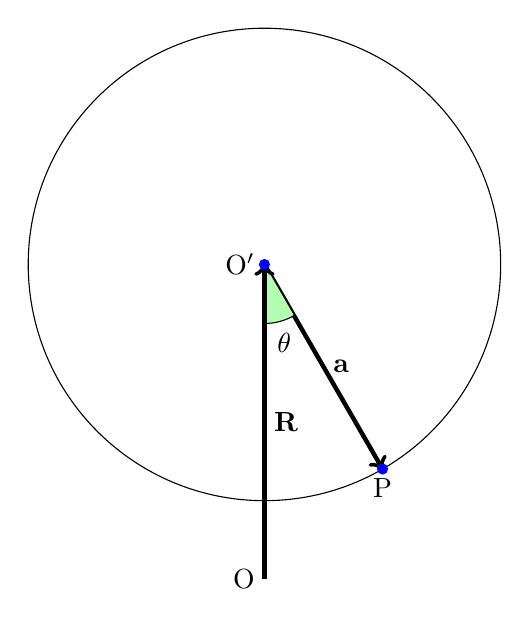
\begin{tikzpicture}
        \coordinate[label=left:{O$'$}] (A) at (0,0);
        \coordinate (B) at (0,-3);
        \coordinate[label=below:{P}] (C) at (3/2,-5.19615242271/2);
        \coordinate[label=right:$\bvec{a}$] (D) at ($ (A)!.5!(C) $);
        \coordinate[label=left:{O}] (E) at (0,-4);
        \coordinate[label=right:$\bvec{R}$] (D) at ($ (A)!.5!(E) $);
        
        \draw (A) circle [radius=3];
        \draw[dashed] (A) -- (B);
        \draw[->,ultra thick] (A) -- (C);
        \draw[fill=green!30] (0,0) -- (270:0.75cm) arc (270:300:0.75cm);
        \draw (1/4,-1) node {$\theta$};
        \draw[->,ultra thick] (E) -- (A);
        
        \fill[blue] (A) circle [radius = 2pt];
        \fill[blue] (C) circle [radius = 2pt];
        \end{tikzpicture}
    \end{figure}
    \\
    
    So, the position of a bead on the wire is described by 
    \begin{align*}
        \bvec{r} &= \bvec{R}+\bvec{a} = h(t)\uv{y} + a(\sin{\theta}\uv{x}+\cos{\theta}\uv{y})\\
        \bvec{v} &= \dot{h}(t)\uv{y}+a(\cos{\theta}\uv{x}-\sin{\theta}\uv{y})
    \end{align*}
    Thus the kinetic energy can be described as 
    \[
        T = \frac{m}{2}(\dot{h}^2(t)-2a\dot{h}(t)\dot{\theta}\sin{\theta}+a^2\dot{\theta}^2)
    \]
    and the potential energy is 
    \[
        V = mga(h(t)-\cos{\theta})
    \]
    This makes our Lagrangian, with time dependence 
    \[
        \lag[\theta,\dot{\theta},t] = \frac{m}{2}(\dot{h}^2(t)-2a\dot{h}(t)\dot{\theta}\sin{\theta}+a^2\dot{\theta}^2) -mgah(t)+mga(h(t)-\cos{\theta})\cos{\theta}
    \]
    But, now we are forced to use the Euler-Lagrange equations and we now have the momentum as
    \begin{align*}
        P_\theta &= \part{\dot{\theta}}{\lag} = -am\dot{h}(t)\sin\theta+ma^2\dot{\theta}\\
        \dot{P_\theta} &= \part{\theta}{\lag} = -am(\ddot{h}(t)\sin{\theta}+\dot{h}(t)\cos{\theta})+ma^2\ddot{\theta} = ma\dot{h}(t)\cos{\theta}-mga\sin{\theta}
    \end{align*}
    But this gives us the ODE
    \[
        \ddot{\theta} = \left(-\frac{g}{a}+\frac{\ddot{h}(t)}{a}\right)\sin\theta
    \]
    Where we see that there is some force that opposes the restoring force from gravity. For example, in the small angle solution, as the angle gets further from the equilibrium point, the force gets bigger depending on the acceleration of $h(t)$. This looks like a driven pendulum. 
    \\
    
    Note: I included an analytic solution to  $\ddot{\theta} = -\frac{g}{a}\sin\theta$ at the end of the assignment. There are also graphics included in the CoCalc that I used to prove to myself that this made sense. 
\end{homeworkProblem}

\pagebreak

\begin{homeworkProblem}
    A point mass $m$ slides without friction along a wire bent into a vertical circle of radius $a$.
    The wire rotates with constant angular velocity $\Omega$ about the vertical diameter, and the apparatus is placed in a uniform gravitational field $\bvec{g}$ parallel to the axis of rotation.
    \begin{itemize}
        \item [(a)]  Construct the lagrangian for the point mass using the angle $\theta$ (angular displacement measured from the downward vertical) as generalized coordinate.
        \item[(b)] Show that the condition for an equilibrium circular orbit at angle $\theta_0$ is $\cos\theta_0 = g/a\Omega^2$. Explain this result by balancing forces in a co-rotating coordinate system.
        \item[(c)] Demonstrate that this orbit is stable against small displacements along the wire and show that the angular frequency of oscillation about the equilibrium orbit is given by $\omega^2 = \Omega^2\sin^2\theta_0$. Hint: Write $\theta = \theta_0 +\eta(t)$, where $\eta(t)$ is a small quantity.
        \item[(d)] What happens if $a\Omega^2 < g$?
    \end{itemize}
    
    \textbf{Solution}\\
    Thinking about the bead sliding down a friction-less wire, in light of the last two problems, we would expect the solutions here to be that of a Foucault pendulum at the north pole of some planet rotating with constant angular velocity $\Omega$. We will use the figure from Problem 4, but we need an addition to our picture to show the effects of a rotation.
    \begin{figure}[h]
        \centering
        \begin{tikzpicture}
        \draw[->, thick] (-.5,0)--(5,0);
        \draw[->, thick] (0,-.5)--(0,5);
        \draw[ultra thick, blue] (0,0)--(3,3);
        \draw (0,0) -- (0:0.75cm) arc (0:45:0.75cm);
        \draw (1.5,1/3) node {$\phi = \Omega t$};
        \end{tikzpicture}
    \end{figure}
    \\
    
    Where the blue line signifies the loop of wire, and $\phi$ is the angle that the loop has rotated by. We will keep our notation of drawing with the origin at it's center. 
    \\
    
    \textbf{Part (a)}\\
    let us define constraint forces that keep the bead rotating with $\phi = \Omega t$ and $r = a$ throughout the dynamics of the system. We will call $F_r$ the force that keeps the bead on the loop, and $F_\phi$ the force that keeps the loop rotating with its constant angular velocity. 
    \[
        T = \frac{m}{2}(\dot{r}^2+r^2\dot{\theta}^2+r^2\sin^2(\theta)\dot{\phi}^2)
    \]
    We know that the only potential effecting the system is a gravitational field pointing uniformly down, thus we can use the gravitational field from the third problem, and 
    \[
        V = -mgr\cos{\theta}
    \]
    But now we have the two constraints 
    \begin{align*}
        &F_r(r-a)\\
        &F_\phi(\phi-\Omega t)
    \end{align*}
    But now the lagrangian becomes 
    \[
        \lag[\dot{r},\dot{\theta},\dot{\phi},r,\theta,\phi,t] = \frac{m}{2}(\dot{r}^2+r^2\dot{\theta}^2+r^2\sin^2(\theta)\dot{\phi}^2)+mgr\cos{\theta}-F_r(r-a)-F_\phi(\phi-\Omega t)
    \]
    But we can now find the momentum for each coordinate, returning 
    \begin{align*}
        P_r &= \part{\dot{r}}{\lag} = m\dot{r}\\
        P_\theta &= \part{\dot{\theta}}{\lag} = mr^2\dot{\theta}\\
        P_\phi &=\part{\dot{\phi}}{\lag} = mr^2\sin^2(\theta)\dot{\phi}\\
        \dot{P_r} &= \part{r}{\lag} = mr\dot{\theta}^2 + mr\sin^2(\theta)\dot{\phi}^2+mg\cos(\theta)-F_r = m\ddot{r}\\
        \dot{P_\theta} &= \part{\theta}{\lag} =ma^2\sin(\theta)\cos(\theta)\Omega^2-mgr\sin(\theta) =  \frac{d}{\dt}[mr^2\dot{\theta}]\\
        \dot{P_\phi} &= \part{\phi}{\lag} = -F_\phi = \frac{d}{\dt}[mr^2\sin^2(\theta)\dot{\phi}]
    \end{align*}
    But we know that we want these constraints are satisfied, $r = a$, $\dot{r} = \ddot{r} = 0$, $\phi = \Omega t$, and $\dot{\phi} = \Omega$. Thus we can use the first and last equations to determine the forces of constraint on the system, and the middle equation will give us the solution we want. 
    \[
        \ddot{\theta} = -\frac{g}{a}\sin{\theta} + \Omega^2\sin{\theta}\cos{\theta}
    \]
    
    \textbf{Part (b)}\\
    Thinking about the equilibrium positions of the wire while it is not moving, we see that the most natural equilibrium positions are at $\theta = 0,\pi/2$. These arise when $\ddot{\theta} = 0$, and we can use the same understanding in this problem. In a more deep understanding, if there was some potential that described the motion of the particle, then we know an equilibrium position exists when the gradient of that potential is zero, i.e.,
    \[
        \grad V\eval_{\bvec{P}} = 0 \iff \part{i}{V_i} = 0 \iff -F = 0
    \]
    So in this case, we can imagine there is some effective potential that is causing the bead move confined to the wire, and with an angular velocity of $\Omega$. When this potential is a minimum, or maximum, the relation above holds, and we have $\ddot{\theta} = 0$, or the relation 
    \[
    \cos{\theta_0} = \frac{g}{a\Omega^2}
    \]
    But now looking at this problem in the rotating frame, we are looking for the point where all the fictitious forces cancel with gravity. But we know that when we are in a frame rotating with the loop, we hope to find the system in a state where there is no acceleration, so we have something like 
    \[
        0 = \bvec{F_g} - m\omega\cp\omega\cp\bvec{r} - 2m\omega\cp\dot{r} - m\dot{\omega}\cp\bvec{r}
    \]
    We know some things about the system namely, $\omega = \Omega$, $r = a$, and $\dot{r} = \ddot{r} = 0$. Thus we have 
    \[
        0 = g\cos{\theta_0} - \Omega\cp\Omega\cp\bvec{a}
    \]
    But since we measure $\theta$ from the downward vertical, the angle between the angular velocity vector and $\bvec{a}$ is nothing but $\pi/2-\theta_0$, and thus we have the relationship 
    \[
        0 = g\cos{\theta_0} - \Omega\cp(a\Omega\cos{\theta_0}) = g\cos{\theta_0} - \Omega^2a\cos^2\theta_0 \iff \cos{\theta_0} = \frac{g}{a\Omega^2}
    \]
    Which is the same result we obtained from the analysis from an inertial frame.
    \\
    
    \textbf{Part (c)}\\
    Suppose we where to perturb the system from $\theta = \theta_0 \to \theta = \theta_0 + \eta(t)$. Then we have the equations 
    
    \[
        \ddot{\eta} = -\frac{g}{a}\sin{(\theta_0 + \eta(t))} + \Omega^2\sin{(\theta_0 + \eta(t))}\cos{(\theta_0 + \eta(t))}
    \]
    But we know that for small angles, 
    \begin{align*}
        \sin(\theta_0+\eta) &= \sin(\theta_0)+\eta\cos(\theta_0)\\
        \cos(\theta_0+\eta) &= \cos(\theta_0)-\eta\sin(\theta_0)
    \end{align*}
    So after plugging this in and canceling our equations, we get 
    \[
        \ddot{\eta} = -\Omega^2\eta \sin^2\theta_0- \Omega^2\eta^2\sin\theta_0\cos\theta_0
    \]
    But since we expanded $\eta$ to degree 1 in our small angle approximations, we do the same here and find the ODE describing a restoring force. This means that any small perturbation away from the equilibrium positions will result in a solution that consists of complex exponentials as opposed to exponential growth or decay. Explicitly, we get
    \[
        \ddot{\eta} = -(\Omega^2 \sin^2\theta_0)\eta = \omega^2\eta
    \]
    With leads to the equation for $\eta$ for all time after the initial perturbation
    \[
        \eta = Re[Ae^{i\omega \eta}]
    \]
    
    \textbf{Part (d)}\\
    Looking back at the ODE result from the Euler-Lagrange equations, we have 
    \[
        a\ddot{\theta} = -g\sin{\theta} + a\Omega^2\sin{\theta}\cos{\theta}
    \]
    Lets break down what this equation physically tells us. Firstly, we note that for the non rotating solution, we just have the first part of the equation, i.e.,
    \[
        a\ddot{\theta} = -g\sin{\theta}
    \]
    If we where to solve the equations in a vacuum without a gravitational field, then we could describe the motion with the following ODE
    \[  
        a\ddot{\theta} = a\Omega^2\sin{\theta}\cos{\theta}
    \]
    And here the equilibrium solution would have $a\Omega^2\sin\theta_1\cos\theta_1 = 0$ and we would observe the bead resting at the top of the loop, $\theta = \pi$. 
    \\
    
    But now we have our system which is in some combination of these two effects. It could be in a state where the gravitational field is week, in which we would assume that the equilibrium state would happen at a higher angle. Now we have the question of what would happen in a relatively strong gravitational field? One such that $a\Omega<g$? In this case, the motion is dominated by the oscillatory motion about the "steady state" solution (I use steady state here to describe the motion with no rotation). But what would this look like? Would the bead all ways find its way to one of these equilibrium positions? or would it's equilibrium be some oscillation about the "steady state equilibrium"? To understand this, let us look us define 
    \[
        \epsilon = \frac{g}{a\Omega^2}
    \]
    When $\epsilon = 1$, the equilibrium position is at $\theta = 0$. When $\epsilon <1$, then we have some real valued theta greater than zero that the bead will "stick" to as it rotates. The one we care about is when $\epsilon>1$. In this case, the equilibrium positions are complex, i.e.,
    \[
        \theta_0 = -i\ln(i\sqrt{1-\epsilon^2}+\epsilon)
    \]
    But this generates a purely imaginary angle, something that is not physically possible. This means that there is no real interpretation of an equilibrium point here. So, we can say that the bead will some form of oscillatory motion and will not have an angle that corresponds to its equilibrium. However, I feel like in this case, the complex $\theta_0$ will correspond to some frequency, and might represent some normal mode of the system. 
\end{homeworkProblem}
\pagebreak
\begin{homeworkProblem}
    Here we will solve the ODE
    \[
        \ddot{\theta} = \frac{g}{a}\sin{\theta}
    \]
    without using the small angle approximation.
    \\
    
    \textbf{Solution}
    Lets start off with reducing the order of the ODE. If you recall, in the 3rd problem, we had no time dependence in the Lagrangian, and thus the Hamiltonian is conserved. This means that we are now open to using the principle we used in the first problem to solve the equation in a simpler form, i.e., 
    \begin{align*}
        \part{t}{\lag-\dot{\theta}P_\theta} &= \part{t}{\frac{m}{2}a^2\dot{\theta}^2+mga\cos{\theta}} = 0\\
        &\frac{m}{2}a^2\dot{\theta}^2+mga\cos{\theta} = a^2E/2(some constant)
    \end{align*}
    Where $E$ is just some constant. To make our lives easier, we will let $m = 1$, and $\omega^2 = 2\frac{g}{a}$ and now we have the equation as nothing but 
    \[
        \dot{\theta}^2-\omega^2\cos{\theta} = E
    \]
    But if we let the initial conditions be $\theta(0) = \theta_0$, and $\dot{\theta}(0) = \dot{\theta}_0$, thus we know that $E = \dot{\theta}_0 - \omega^2\cos{\theta_0}$. So now the differential equation becomes 
    \[
        \dot{\theta}^2=\omega^2\cos{\theta}+\dot{\theta}_0 - \omega^2\cos{\theta_0}
    \]
    But by double angle trigonometric identities, letting $\Omega = 2\omega$, and letting $k = \sin(\theta_0/2)$, we reduce our differential equation to something that is separable and first order. Where we will let the initial velocity be zero. 
    \[
        \dot{\theta} = \sqrt{\omega}\sqrt{k^2-\sin^2(\theta/2)}
    \]  
    But now we have the integral 
    \[
        \int_o^{\theta_0}\sqrt{k^2-\sin^2(\theta/2)}^{-1}\dt = \sqrt{\omega}\int_{0}^{\theta_0}\dt
    \]
    but, the right hand side of the integral is just the time it takes to for the pendulum to make one quarter of is period time $\tau$. Similarly, we can make a substitution and let $\sin{\theta/2} = k\sin{\vartheta}$, and $k\cos{\vartheta}\mathrm{d}\vartheta = 1/2\cos{\theta/2}\mathrm{d}\theta$. But using Pythagorean identity this gives us the relationship 
    \[
        \cos{\theta/2} = \sqrt{1-\sin^2\theta/2} = \sqrt{1-k^2\sin^2\vartheta}
    \]
    So the substitution becomes 
    \[
        \mathrm{d}\theta = \frac{2k\cos{\vartheta}}{\sqrt{1-k^2\sin^2(\vartheta)}}\mathrm{d}\vartheta
    \]
    so our integration becomes 
    \[
        \frac{\sqrt{\omega}}{4}\tau = \int_{0}^{\pi/2}\frac{1}{k\cos\vartheta}\frac{2k\cos{\vartheta}}{\sqrt{1-k^2\sin^2\vartheta}}\mathrm{d}\vartheta
    \]
    so now we have an equation for the period time as nothing but 
    \[
        \tau = \frac{8}{\sqrt{\omega}}\int_0^{\pi/2}\frac{\mathrm{d}\vartheta}{\sqrt{1-k^2\sin^2\vartheta}} 
    \]
    And we now have the period time for our bead sliding along the loop of wire in terms of the complete elliptic integral of the first kind. And lets plug back in the constants that we know to get the equation in terms of known constants. 
    \[
        \tau = 4\sqrt{a/g}K(k)
    \]
    where $K(k)$ is nothing but the complete elliptic integral of the first kind. 
    \\
    
    \textbf{Part 2}\\
    If we instead wanted to solve this equation using the small angle approximation of $\sin{\theta} = \theta$, then we would be doing a small oscillations approximation, and we have the ODE
    \[
        \ddot{\theta} = -\frac{g}{a}\theta
    \]
    we guess the solutions for $\theta$ are the real part of some complex exponential, $\vartheta = Ae^{i\omega t}$, where the amplitude holds the initial condition of the bead, ie.e
    \[
        \theta = Re[\vartheta] = Re[\alpha e^{i\beta}e^{i\omega t}]
    \]
    Plugging this into the ODE, we get $\omega^2 = g/a$, and $\alpha$ and $\beta$ are determined by the initial conditions of the problem. 
\end{homeworkProblem}
\end{document}
%----------------------------------------------------------------------------------------------------------------------------------------------------------------------------------
%----------------------------------------------------------------------------------------------------------------------------------------------------------------------------------
%----------------------------------------------------------------------------------------------------------------------------------------------------------------------------------
